\section{Проектирование информационной системы вокзала}

\subsection{Разработка функционала системы}

Для разработки данной информационной системы использовался уже раннее представленный язык программирования \textit{C++}. В качестве \textit{IDE (integrated development environment)} для работы с этим языком был выбран \textit{Clion}. Эта программа предоставляет все необходимые возможности для комфортной разработки программного средства. 

Данный язык был выбран так же с учетом того, что он предоставляет ряд готовых решений. Поэтому во время выполнения курсового проекта использовались следующие библиотеки:

\begin{itemize}
    \item библиотека \textit{iostream} -- предоставляет инструменты для организации ввода и вывода данных в языке программирования C++. Основные компоненты включают \textit{std::cin} для ввода, \textit{std::cout} для вывода, а также \textit{std::cerr} для отображения ошибок.
    \item библиотека \textit{limits} -- содержит шаблонный класс \textit{std::numeric\_limits}, предоставляющий информацию о свойствах числовых типов, таких как максимальное и минимальное значения, точность, поведение при переполнении.
    \item библиотека \textit{sqlite3.h} -- библиотека для работы с базой данных SQLite. Предоставляет функции и методы для создания, изменения, удаления таблиц и записи данных, а также выполнения SQL-запросов.
    \item библиотека \textit{utility} -- включает полезные инструменты, такие как класс \textit{std::pair} для создания пары значений и функции для работы с ними. 
    \item библиотека \textit{vector} -- предоставляет контейнер \textit{std::vector}, представляющий собой динамический массив с удобным интерфейсом для добавления, удаления и доступа к элементам.
\end{itemize}

Проектирование информационной системы предусматривало её работу в терминале на платформе семейства \textit{Unix}, что обеспечивает стабильную и эффективную работу приложения в средах, поддерживающих соответствующие командные оболочки. Учитывая, что операционные системы \textit{Windows} по умолчанию не включают стандартных инструментов для работы с терминалом \textit{Unix}, использование программы в таких системах возможно только при установке дополнительных программных средств, таких как \textit{Windows Subsystem for Linux (WSL)} или эмуляторов терминала.

Разрабатываемая система имеет разграничение прав доступа между двумя типами пользователей: обычным пользователем и администратором. Каждому пользователю предоставляются различные функции в зависимости от его роли в системе. Обычный пользователь имеет доступ к ограниченному набору функций, связанных с обработкой и управлением билетами. Администратор же, помимо этих возможностей, обладает правами на управление станциями, поездами, вагонами и маршрутами, а также на выполнение более широких операций с билетами.

Обычный пользователь системы может выполнять следующие действия:
\begin{itemize}
    \item Просмотр списка билетов: пользователь может увидеть все зарегистрированные билеты и информацию о них.
    \item Создание билета: пользователь может создать новый билет для себя или другого пассажира.
    \item Удаление билета: пользователь может удалить выбранный билет из системы.
\end{itemize}

Администратор обладает дополнительными правами, включая все функции обычного пользователя, а также:
\begin{itemize}
    \item Управление станциями: администратор может добавлять, просматривать и удалять станции.
    \item Управление поездами: администратор может создавать, просматривать и удалять поезда.
    \item Управление вагонами: администратор имеет возможность добавлять, просматривать и удалять вагоны в поездах.
    \item Управление местами: администратор может просматривать и изменять доступные места в поездах.
    \item Управление маршрутами: администратор может просматривать, добавлять и изменять маршруты.
    \item Работа с билетами: администратор имеет те же возможности, что и обычный пользователь, но дополнительно может изменять или удалять билеты других пользователей.
\end{itemize}


Каждая из этих функций организована в виде меню, в котором пользователь или администратор может выбрать нужное действие для управления системой.

\subsection{Разработка иерархии классов}

Исходя из того, какие действия будет выполнять информационная система и какими данными будет оперировать создаются следующие классы:

\begin{itemize}
    \item Класс \textit{System} -- содержит функции для запуска системы и входа в аккаунт.
    \item Класс \textit{Database} -- содержит функции для работы с базой данных.
    \item Класс \textit{Entity} -- абстрактный класс, содержащий общие функции для работы классов пользователей системы.
    \item Класс \textit{Admin} -- содержит функции для работой с классом \textit{Database}, характерные для администратора.
    \item Класс \textit{User} -- содержит функции для работой с классом \textit{Database}, характерные для пользователя.
\end{itemize}

Иерархия классов представлена на рисунке \ref{fig:struct_classes}:

\begin{figure}[h]
    \centering
    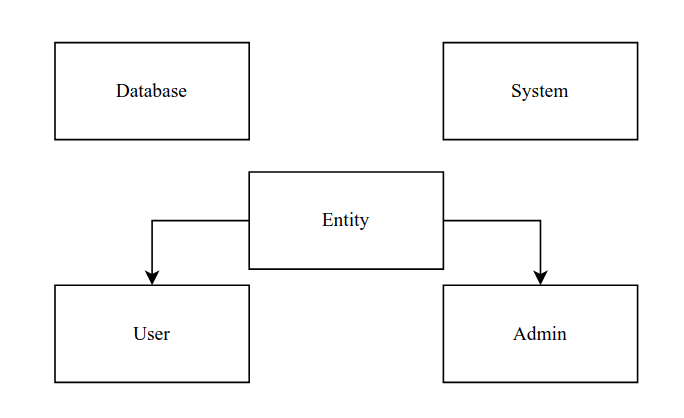
\includegraphics[width=1\textwidth]{struct_classes.png}
    \caption{Иерархия классов}
    \label{fig:struct_classes}
\end{figure}


\subsection{Хранение данных}

В качестве базы данных будет использоваться \textit{SQLite}. \textit{SQLite} — это встраиваемая база данных, которая не требует отдельного сервера и обеспечивает высокую производительность и простоту использования. Она хранит всю информацию в одном файле и идеально подходит для приложений, которые нуждаются в компактном и эффективном хранилище данных. В связке с \textit{C++} и \textit{CLion SQLite} позволяет быстро и легко интегрировать функционал работы с базой данных, что делает её отличным выбором для разработки приложений с базовыми потребностями в хранении данных.

Структура базы данных представлена на рисунке \ref{fig:struct_db}.\\

\begin{figure}[h]
    \centering
    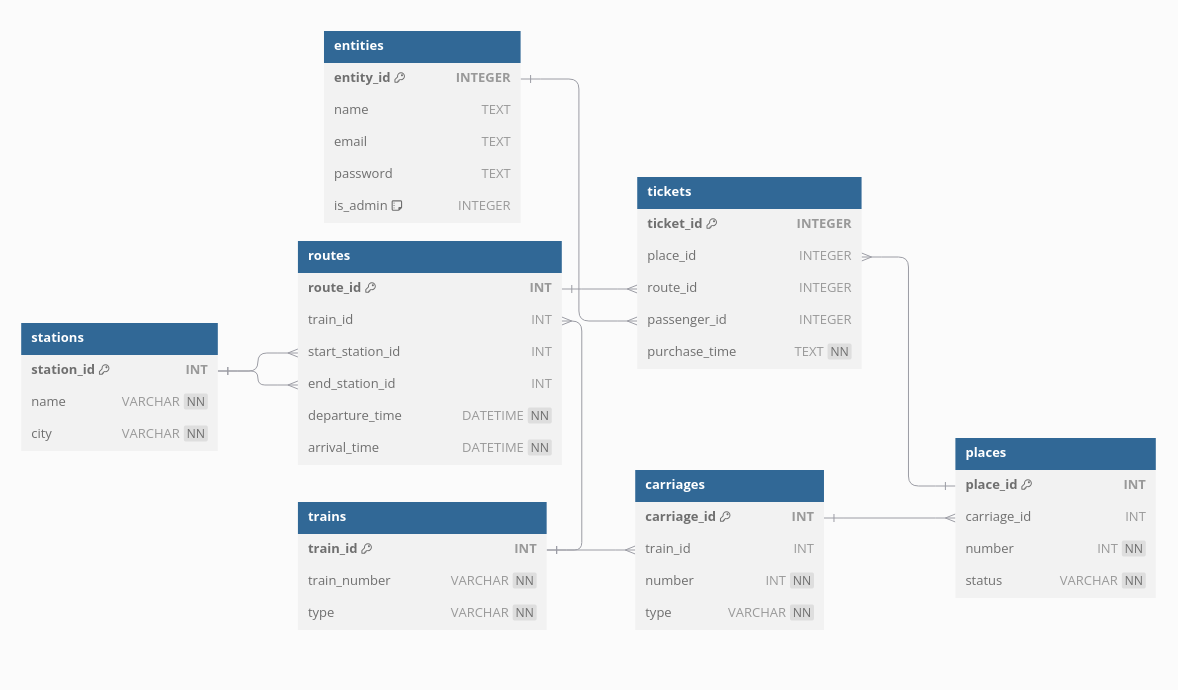
\includegraphics[width=1\textwidth]{db_structure.png}
    \caption{Структура базы данных}
    \label{fig:struct_db}
  \end{figure}

  Структура базы данных организована с использованием нескольких таблиц, каждая из которых отвечает за хранение определенной информации, связанной с вокзалом, поездами, вагонами, местами и билетами.

  \begin{itemize}
    \item Таблица \textit{stations} — содержит информацию о станциях. Каждая станция имеет уникальный идентификатор (\textit{station\_id}), название (\textit{name}) и город, в котором она расположена (\textit{city}).
    \item Таблица \textit{trains} — хранит информацию о поездах. Каждому поезду присваивается уникальный идентификатор (\textit{train\_id}), номер поезда (\textit{train\_number}) и его тип (\textit{type}).
    \item Таблица \textit{carriages} — предназначена для хранения информации о вагонах. В каждом вагоне хранится уникальный идентификатор (\textit{carriage\_id}), идентификатор поезда, к которому принадлежит вагон (\textit{train\_id}), номер вагона (\textit{number}) и его тип (\textit{type}). В таблице также используется внешний ключ, который связывает вагоны с поездами, с условием удаления вагонов при удалении соответствующего поезда.
    \item Таблица \textit{places} — хранит информацию о местах в вагонах. Каждый элемент в таблице включает уникальный идентификатор места (\textit{place\_id}), идентификатор вагона, к которому оно принадлежит (\textit{carriage\_id}), номер места (\textit{number}) и статус места (\textit{status}). Также присутствует внешний ключ, который связывает места с вагонами, с условием удаления мест при удалении соответствующего вагона.
    \item Таблица \textit{routes} — содержит информацию о маршрутах поездов, включая идентификатор маршрута (\textit{route\_id}), идентификатор поезда, который следует по маршруту (\textit{train\_id}), идентификаторы начальной и конечной станций (\textit{start\_station\_id}, \textit{end\_station\_id}), а также время отправления и прибытия (\textit{departure\_time}, \textit{arrival\_time}). В таблице используются внешние ключи, связывающие маршруты с поездами и станциями.
    \item Таблица \textit{entities} — хранит данные о пользователях системы. Каждый пользователь имеет уникальный идентификатор (\textit{entity\_id}), имя (\textit{name}), электронную почту (\textit{email}), пароль (\textit{password}) и флаг администратора (\textit{is\_admin}).
    \item Таблица \textit{tickets} — хранит данные о билетах. Каждый билет имеет уникальный идентификатор (\textit{ticket\_id}), идентификатор места, на которое был продан билет (\textit{place\_id}), идентификатор маршрута, на котором используется билет (\textit{route\_id}), идентификатор пассажира (\textit{passenger\_id}), который приобрел билет, и время покупки билета (\textit{purchase\_time}). В таблице также используются внешние ключи, связывающие билеты с местами, маршрутами и пассажирами.
\end{itemize}
